\chapter{Proposta de Desenvolvimento}

\section{Ambiente para Aprendizado e Prática de Técnicas de Segurança
Ofensiva em Aplicações Web Vulneráveis}

Existe uma similaridade entre a OWASP Broken, a Mutillidae e o ambiente proposto neste trabalho, os tipos de falhas encontrados nestas duas máquinas são muito semelhantes às falhas que serão desenvolvidas neste ambiente, porém a grande diferença é que este ambiente será desenvolvido em Docker com a intenção de facilitar a instalação e diminuir a ocupação de dados alocados em máquina.

O ambiente será desenvolvido com base em uma imagem Linux Ubuntu 22.04, para que possam ser exploradas não apenas falhas em aplicações web, mas falhas em aplicações web que levem a falhas em nível de sistemas operacional. Mesmo que isto custe um pouco mais de recursos em contra-ponto a uma aplicação que usaria \textit{docker-compose} para manter os serviços rodando separadamente.

As aplicações executadas dentro do Docker estarão por padrão disponíveis apenas ao Host de forma local para evitar que as vulnerabilidades sejam exploradas por atacantes.

\begin{figure}[!htb]
     \centering
     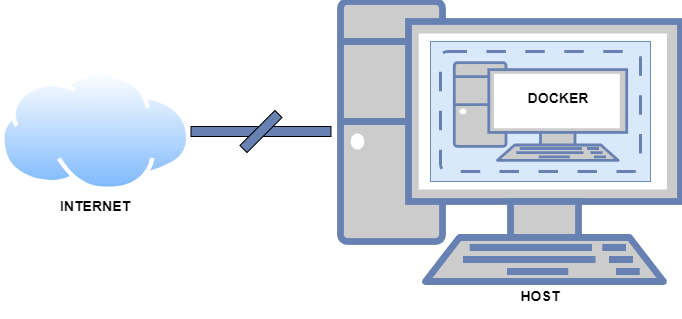
\includegraphics[width=15cm]{proposal.png}
     \caption{Ambiente proposto}
     \label{Label de referência para a imagem}
\end{figure}

A imagem docker do Ubuntu será alterada para conter alguns serviços, sendo os principais estes três: back-end sendo desenvolvido em NodeJS, front-end desenvolvido em JavaScript com React e um banco de dados com SQLite.
Alguns microsserviços também estarão disponíveis para explorar falhas pontuais e estão indicadas corretamente pelo front-end da aplicação.

\section{Vulnerabilidades selecionadas}

\subsection{CWE-23: Relative Path Traversal}

Ocorre quando existem entradas externas para a criação do \textit{path} de um determinado diretório, porém a entrada não é neutralizada e valores como "../" conseguem participar do path. Isso pode permitir por exemplo que diretórios indevidos sejam acessados como entradas do estilo "../../../../etc/passwd".

\subsection{CWE-319: Cleartext Transmission of Sensitive Information}

Ocasionada quando o sistema realiza a transmissão de dados sensíveis ou críticos em texto plano e permite que usuários não autorizados interceptem o dado.

\subsection{CWE-328: Use of Weak Hash}

Quando o algoritmo de Hash não tem como produto um resumo forte o suficiente, ele fica vulnerável a ataques que encontrem a valor original através de ataques de pré-imagem, 2ª pré-imagem ou ataques de aniversário.

\subsection{CWE-74: Improper Neutralization of Special Elements in Output Used by a Downstream Component}

Vulnerabilidade de injeção baseada na falta de neutralização de caracteres especiais nos valores de entrada que podem alterar a forma de interpretação e execução da aplicação.

\subsection{CWE-209: Generation of Error Message Containing Sensitive Information}

Um designe inseguro de aplicação que permite que o usuário veja informações sobre o ambiente, os usuários e dados relacionados através dos erros gerados na aplicação.

\subsection{CWE-613: Insufficient Session Expiration}

Falha na aplicação que permite acesso por sessões antigas ou apenas com o ID de acesso.

\subsection{CWE-565: Reliance on Cookies without Validation and Integrity Checking}

Acontece quando a aplicação depende dos dados nos Cookies para a realização de operações críticas, mas a aplicação não garante que os Cookies são do usuário da sessão.